\chapter{Performance Bottlenecks in \CZTS}

\section{Thermodynamic Disordering of Cu \& Zn Ions in \CZTS}
\subsection{Spatial Extent of Disorder Amongst Cu and Zn Cations}
\begin{itemize}
\item Recovery of kesterite ground state at T=50k? (Cu-Zn and Cu-Sn layers, see lab book pg 2): visuals of structure in VESTA and RDF of Cu-Zn and Cu-Sn pairs
\item Visuals of configs from eris and RDFs across T range 
\end{itemize}
\subsection{Band Tailing due to Fluctuations in Electrostatic Potential}
R plots for distributions of electrostatic potential of Sn

\section{Formation Energy of Sulfur Vacancies}
We investigate the formation energy of charge neutral sulfur vacancies (V$_{S}^{0}$) as a function of the sulfur chemical potential, which itself is a function of temperature and pressure. We therefore can assess the formation energy of the vacancy under typical annealing conditions. Work from Scragg et al showed that annealing out Cu and Zn disorder can be a very time consuming process, therefore for most practical purposes some disorder will be `frozen in' after annealing. Typical annealing conditions for { \CZTS } are at ?? K and it has been shown that lower pressures are more optimal for the sulfide (whereas higher pressures are better for the selenide) **cite Adam?**. This is due to the allotropes of S?\\

On -going calculations are being performed for the charged sulfur vacancies (V$_{S}^{+1}$ and V$_{S}^{+2}$) so that the minimum energy defect, accounting for all possible charge states, across the temperature and pressure range can be determined.

\begin{figure}[h!]
  \centering
    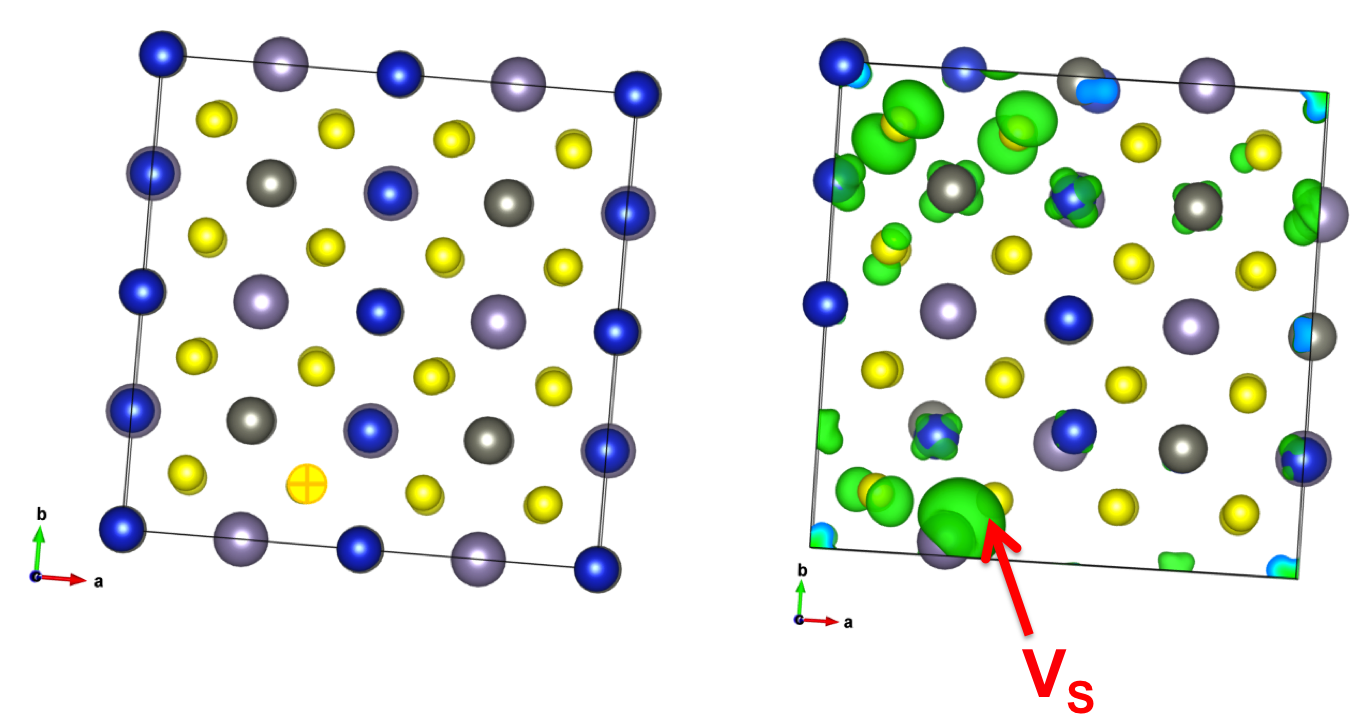
\includegraphics[width=0.9\textwidth]{figures/V_S-neutral-PARCHG.png}
    \caption{Perfect {\CZTS } supercell with S anion removed to form a sulfur vacancy (V$_S$) indicated by a crosshair (left) and the calculated partial charge density of two excess electrons present for the charge neutral V$_S$ (right).}
  \label{V_S-neutral-PARCHG}
\end{figure}

\section{Intrinsic Band Gap Broadening from Lattice Vibrations}
 
